\documentclass[hyperref={colorlinks = true,linkcolor = blue, citecolor=blue,urlcolor=blue}]{beamer}  
\usetheme{default}

\usepackage{amsthm,amsmath,amssymb}
\usepackage{dsfont}
\usepackage{graphicx}
\usepackage{natbib}
\usepackage[space]{grffile}
\usepackage{booktabs}


\title{The Impact of Natural Disasters on Education: \\ Evidence from Standardized Testing}
\author{Gregor Steiner}
\date{July 11, 2022}

\begin{document}
		
\begin{frame}[plain]
    \maketitle
\end{frame}

\begin{frame}{Motivation: Natural disasters over time}
	\begin{figure}[!h]
		\centering
		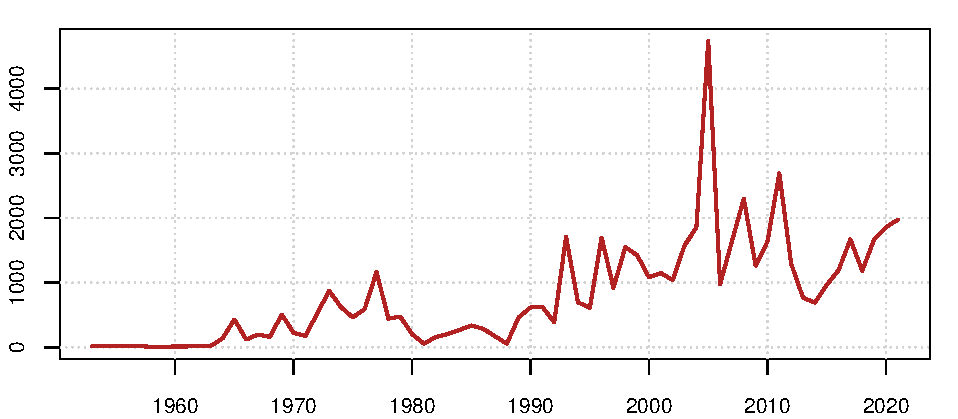
\includegraphics[scale=0.7]{"../Code & Data/DisasterCount.pdf"}
		\caption{Number of county-level natural disasters by year}
		\label{DisasterCount}
	\end{figure}
\end{frame}

\begin{frame}{Motivation: Distribution of natural disasters}
	\begin{figure}[!h]
		\centering
		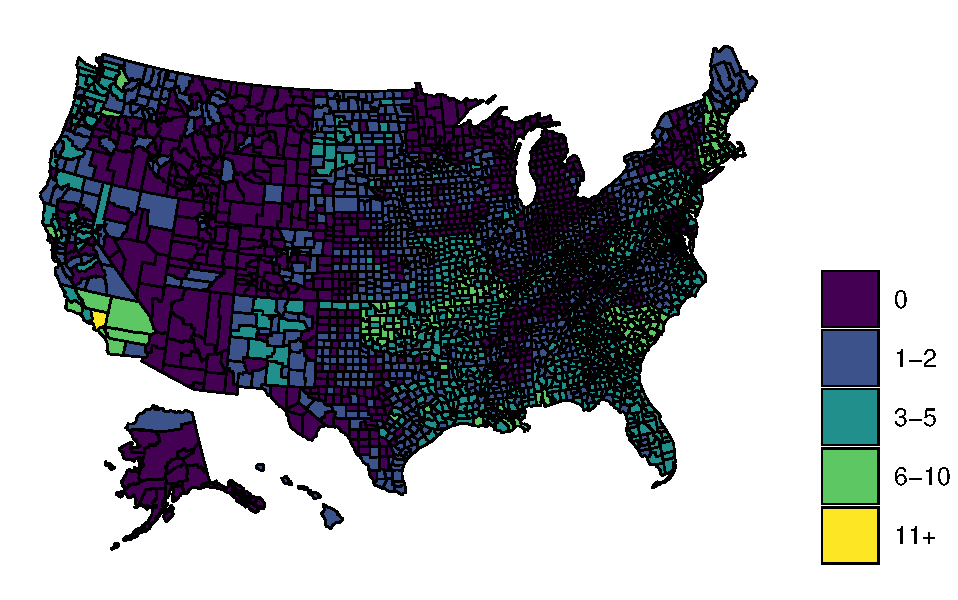
\includegraphics[scale=0.65]{"../Code & Data/DisasterMap.pdf"}
		\caption{Number of declared natural disasters in school years 2008-09 through 2017-18}
		\label{DisasterMap}
	\end{figure}
\end{frame}

\begin{frame}{Research question}
	I exploit quasi-random variation in natural disaster exposure in the United States to answer two questions:
	\begin{itemize}
		\item \textbf{What is the causal effect of natural disasters on academic achievement as measured by standardized test scores?}
		\item What is the role of federal disaster assistance? Which counties apply for assistance?
	\end{itemize}
	\textbf{Why is this important?}\\
	Negative effects in education affect earnings
	potential $\implies$ Inequality in disaster risk exposure could exacerbate economic inequality
\end{frame}

\begin{frame}{Data}
	\begin{itemize}
		\item \textbf{Natural disasters}:
		\begin{itemize}
			\item Federal Emergency Management Agency (FEMA) declarations 
			\item Storms from the National Weather Service (NWS)
			\item Daily temperature data from the Global Historical Climatology Network
		\end{itemize}
		\item \textbf{Standardized testing outcomes} from the Stanford Education Data Archive \citep{SEDA}:
		\begin{itemize}
			\item Cohort standardized average scores by county in Mathematics \& Reading Language Arts (RLA)
			\item Grades 3 through 8 for schoolyears 2008-09 to 2017-18
		\end{itemize}
		\item \textbf{Public Assistance applications and payments} from FEMA
	\end{itemize}
\end{frame}

\begin{frame}{Distribution of mean test scores by subgroup}
	\begin{figure}[!h]
		\centering
		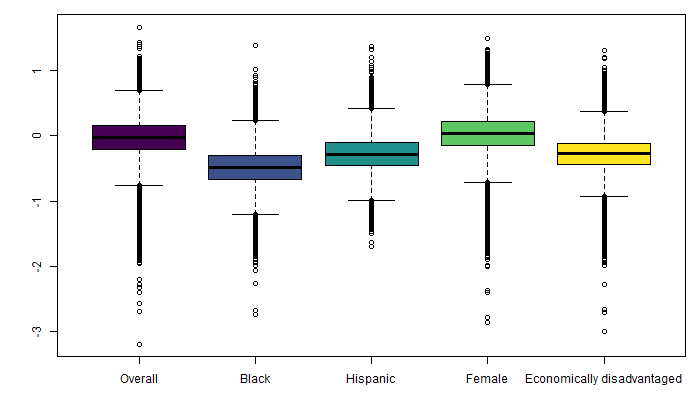
\includegraphics[scale=0.68]{"../Code & Data/DepVarsBoxplot.pdf"}
		\caption{Boxplots of mean test scores by subgroup}
		\label{DepVarsBoxplot}
	\end{figure}
\end{frame}


\begin{frame}{When do counties apply for assistance?}
	\small
	\begin{table}

\caption{\label{tab:AppsByType}Share of counties that applied for federal assistance following a disaster by disaster type (schoolyears 2016-17 and 2017-18)}
\centering
\begin{tabular}[t]{lrr}
\toprule
  & Number of Cases & Applied for Assistance (in \%)\\
\midrule
Coastal Storm & 3 & 33.33\\
Dam/Levee Break & 3 & 0.00\\
Fire & 100 & 11.00\\
Flood & 270 & 41.85\\
Hurricane & 1217 & 23.25\\
Mud/Landslide & 22 & 50.00\\
Severe Ice Storm & 20 & 0.00\\
Severe Storm(s) & 164 & 28.66\\
Snow & 36 & 8.33\\
Tornado & 29 & 79.31\\
\addlinespace
Total & 1864 & 26.39\\
\bottomrule
\end{tabular}
\end{table}

\end{frame}

\begin{frame}{Which counties apply for assistance?}
	\begin{figure}[!h]
		\centering
		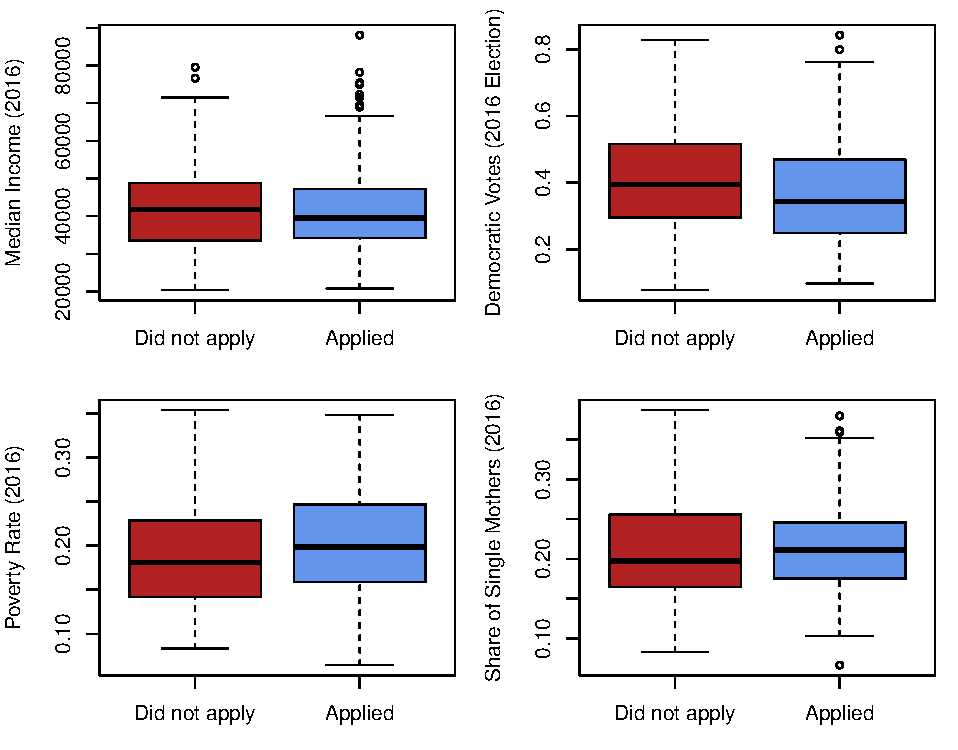
\includegraphics[scale=0.58]{"../Code & Data/AssistanceCovBoxplot.pdf"}
		\caption{Boxplots by application status}
		\label{AssistCovBoxplot}
	\end{figure}
\end{frame}

\begin{frame}{Empirical Strategy}
	\begin{itemize}
		\item Event-study design:
		\begin{align*}
			y_{i, t, g} &= \beta_{-5}  \mathds{1}\{t - E_i \leq 5\} + \sum_{l = -4, \; l \neq -1}^{8} \beta_l \mathds{1}\{t - E_i = l\} \\ &+ \alpha_i + \lambda_t + \zeta_g + \varepsilon_{i, t, g}
		\end{align*}
		\item Treatment begins in the period of first disaster ($E_i$) and is absorbing (staggered adoption)
		\item But: Always-treated (i.e. disaster in the first year) counties are dropped
		\item Never-treated counties act as the baseline
		\item Standard-errors clustered at the county level \citep{Abadie_2017, Sun_2021}
	\end{itemize}
\end{frame}

\begin{frame}{Empirical Strategy: Identification}
	\begin{itemize}
		\item Natural disasters are plausibly independent of unobserved determinants of test scores conditional on location and year
		\item Heterogenous treatment effects $\implies$ simple TWFE is inadequate \citep{deChaisemartin_2020, Sun_2021}
		\item Solution: Interaction-Weighted Estimator (IW) by \cite{Sun_2021}
		\item Identifying Assumptions: Parallel Trends \& No Anticipatory Behavior
		\item IW consistently estimates a weighted average of cohort average treatment effects on the treated (CATT)
	\end{itemize}
\end{frame}

\begin{frame}{Main Results: FEMA}
	\begin{figure}[!h]
		\centering
		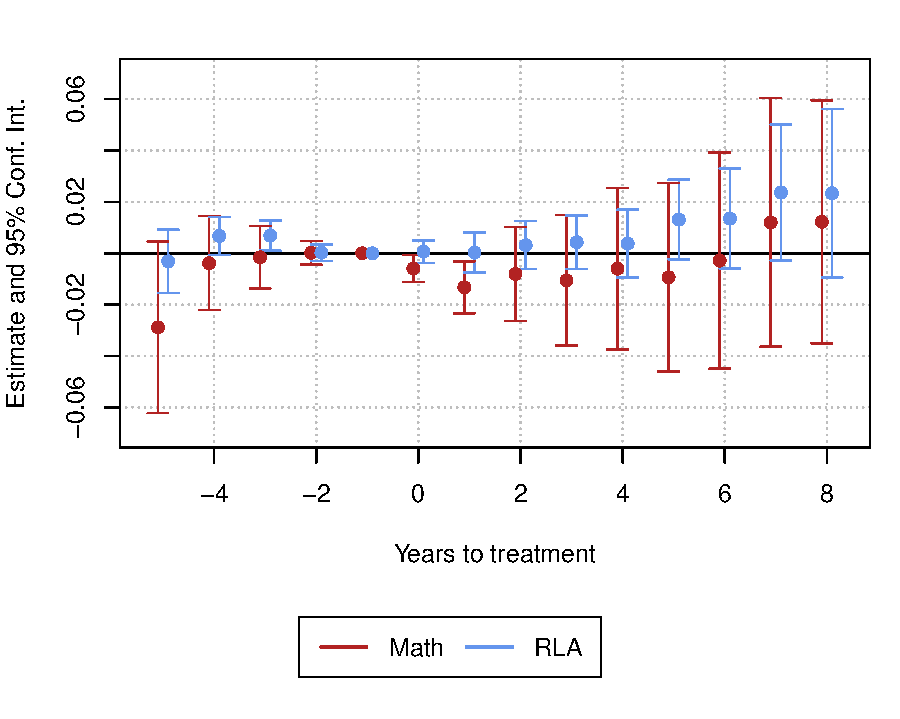
\includegraphics[scale=0.45]{"../Code & Data/ResultsPlotPresentation.pdf"}
		\caption{Dynamic Treatment effects in relative time: FEMA disaster data}
	\end{figure}
\end{frame}


\begin{frame}{Main Results: Storms}
	\begin{figure}[!h]
		\centering
		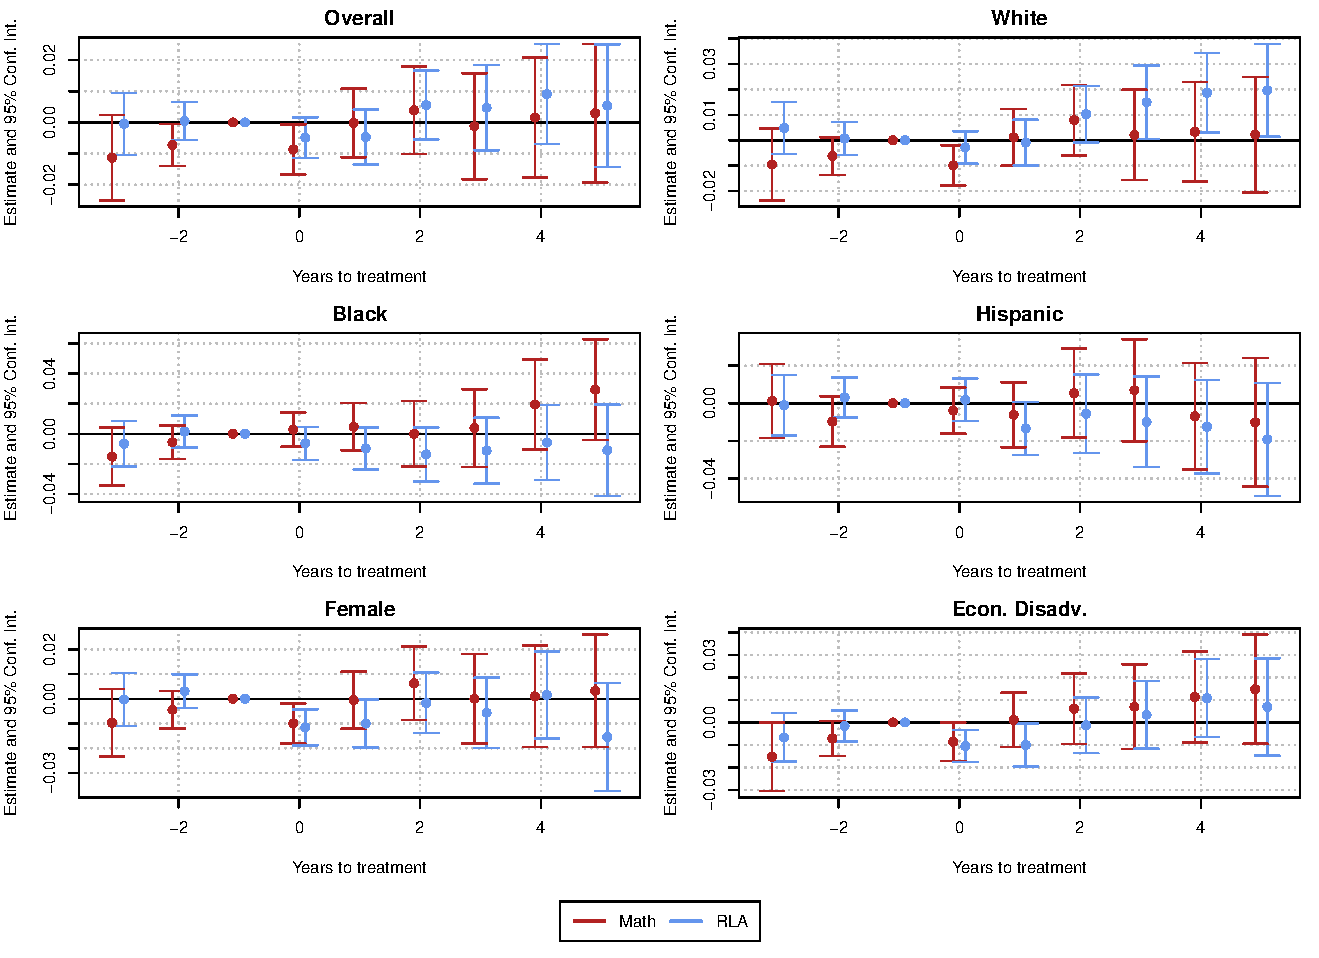
\includegraphics[scale=0.45]{"../Code & Data/ResultsPlotStormPresentation.pdf"}
		\caption{Dynamic Treatment effects in relative time: NWS storms data}
	\end{figure}
\end{frame}


\begin{frame}{Main Results: FEMA (Storms only)}
	\begin{figure}[!h]
		\centering
		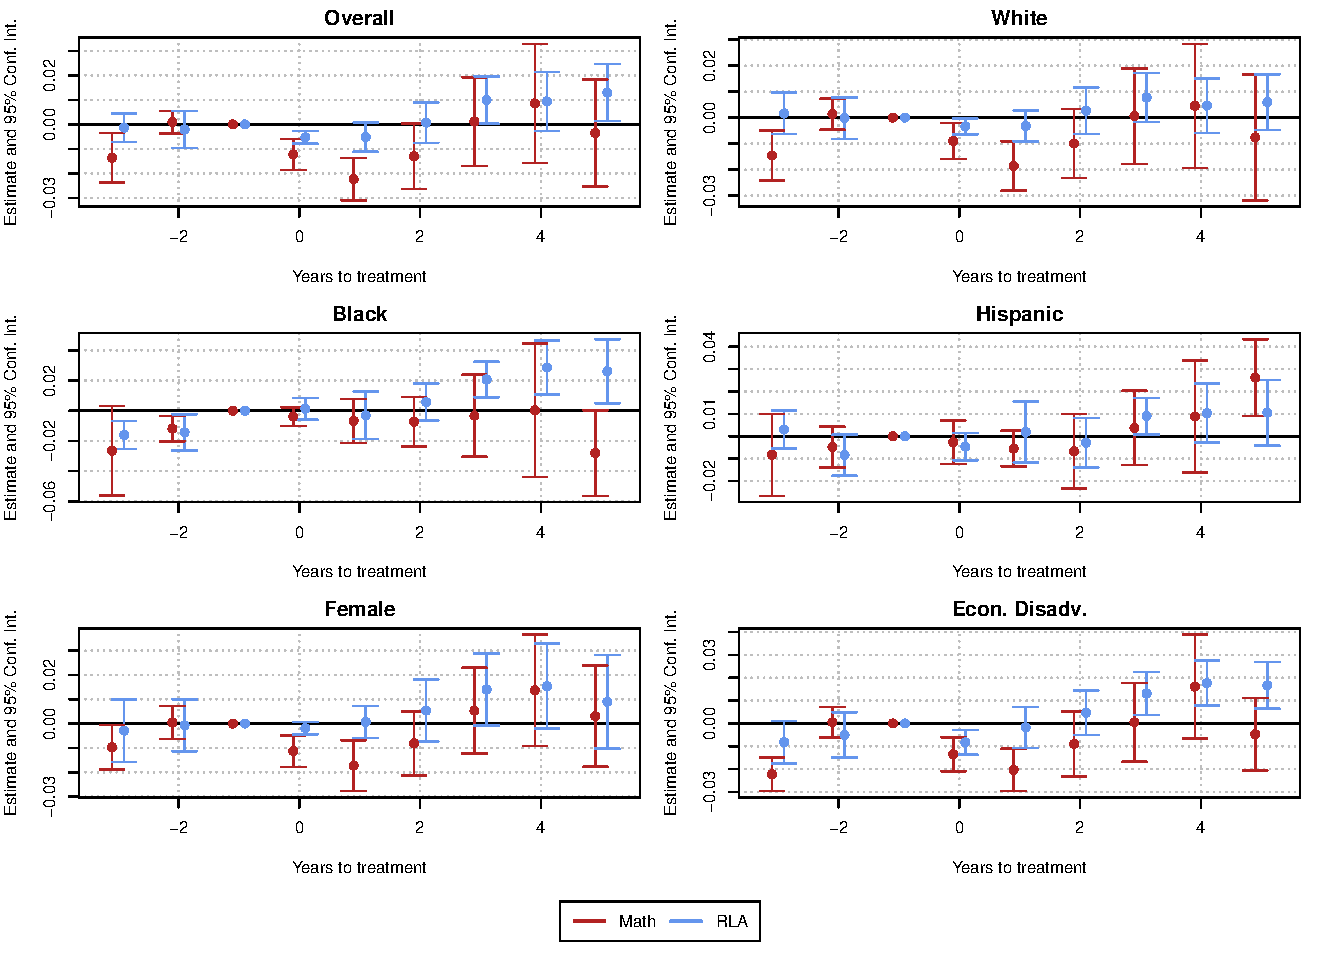
\includegraphics[scale=0.45]{"../Code & Data/ResultsPlotFEMAStormPresentation.pdf"}
		\caption{Dynamic Treatment effects in relative time: FEMA data (storms only)}
	\end{figure}
\end{frame}


\begin{frame}{Are these results driven by changes in county composition?}
	\begin{figure}[!h]
		\centering
		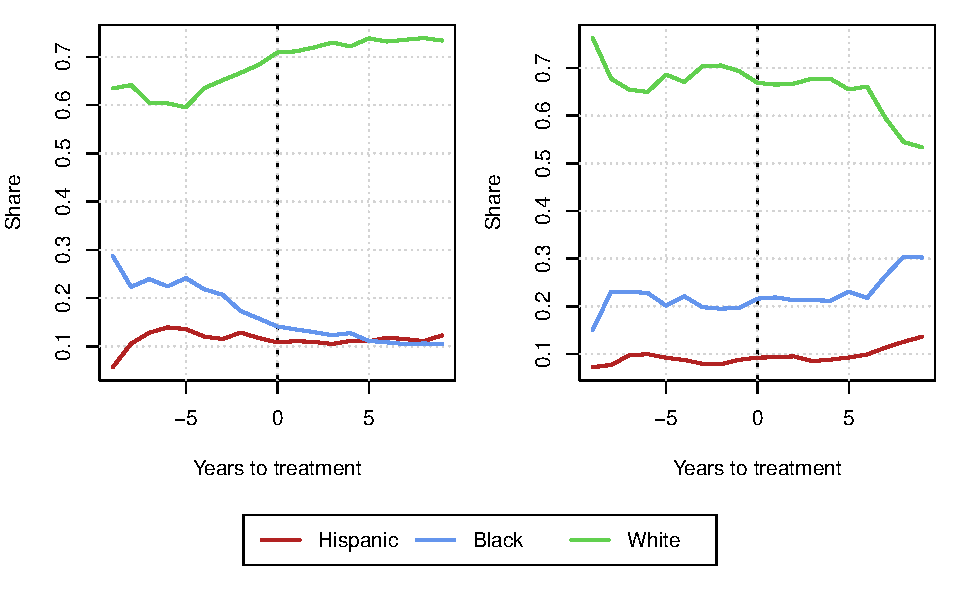
\includegraphics[scale=0.6]{"../Code & Data/EthnicComposition.pdf"}
		\caption{Aggregated ethnic shares by treatment timing based on FEMA disasters (left) and on NWS storms (right)}
		\label{EthnicComposition}
	\end{figure}
\end{frame}

\begin{frame}{Empirical Strategy: Heat}
	\begin{itemize}
		\item A binary treatment indicator is not well-suited to measure cumulative heat exposure. Following \cite{Goodman_2020}, I use two measures:
		\begin{itemize}
			\item Average daily maximum temperature
			\item Number of days above 30°C
		\end{itemize}
		\item Linear model with county, year, and grade fixed effects:
		\begin{align*}
			y_{i, t, g} = \beta H_{i, t} + \alpha_i + \lambda_t + \zeta_g + \varepsilon_{i, t, g}
		\end{align*}
		\item Conditional on location and year, heat exposure is exogenous
		\item Interesting marginal interpretation of $\beta$: What is the effect of a 1°C hotter school year or of one additional	day above 30°C on average test scores?
	\end{itemize}
\end{frame}

\begin{frame}{Heat: Average daily maximum temperature}
	\begin{figure}[!h]
		\centering
		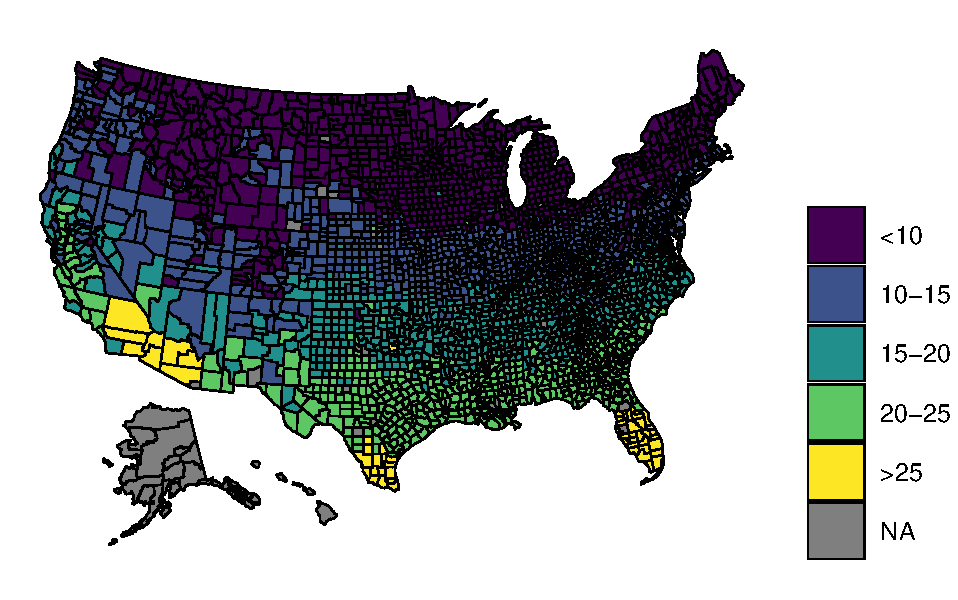
\includegraphics[scale=0.65]{"../Code & Data/HeatMapTemp.pdf"}
		\caption{Average daily maximum temperature (in °C) in school years 2008-09 through 2017-18}
		\label{HeatMapTemp}
	\end{figure}
\end{frame}

\begin{frame}{Heat: Average number of days above 30°C}
	\begin{figure}[!h]
		\centering
		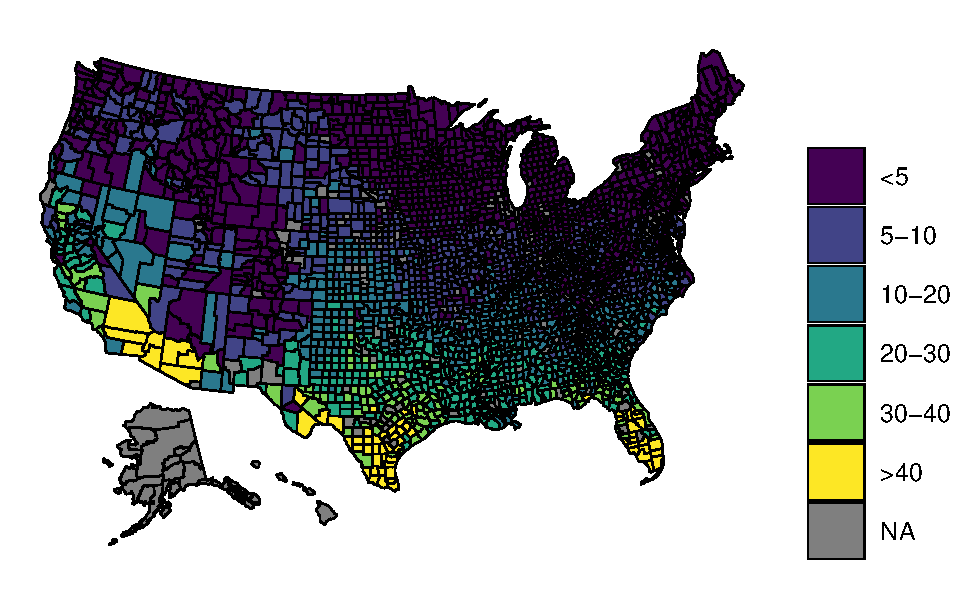
\includegraphics[scale=0.65]{"../Code & Data/HeatMapDays.pdf"}
		\caption{Average number of days above 30°C in school years 2008-09 through 2017-18}
		\label{HeatMapDays}
	\end{figure}
\end{frame}

\begin{frame}{Heat Results}
	\begin{itemize}
		\item No significant overall effect, but minorities seem to be more affected
		\item Possibly driven by unequal access to air-conditiong \citep{Goodman_2020}
	\end{itemize}
	
\begin{tabular}{lllllll}
\toprule
  & Overall & White & Black & Hispanic & Female & Econ. Disadv.\\
\midrule
Max. Temp. (Math) & $-0.0007$ & $-0.0002$ & $-0.0006$ & $-0.0021^{***}$ & $-0.001^{***}$ & $-0.0011^{***}$\\
 & $(0.0003)$ & $(0.0004)$ & $(0.0008)$ & $(0.0006)$ & $(0.0004)$ & $(0.0004)$\\
\addlinespace
Max. Temp. (RLA) & $-0.0001$ & $0.0005$ & $-0.0015^{***}$ & $-0.0011^{***}$ & $-0.0002$ & $-0.0004$\\
 & $(0.0003)$ & $(0.0003)$ & $(0.0007)$ & $(0.0006)$ & $(0.0003)$ & $(0.0003)$\\
\addlinespace
Days ab. 30 (Math) & $-0.000169$ & $-0.000111$ & $0.000033$ & $-0.000196$ & $0.000003$ & $0.000003$\\
 & $(0.000089)$ & $(0.000096)$ & $(0.000143)$ & $(0.000136)$ & $(0.000095)$ & $(0.000096)$\\
\addlinespace
Days ab. 30 (RLA) & $-0.000095$ & $-0.000178^{***}$ & $-0.00014$ & $-0.000483^{***}$ & $-0.000202^{***}$ & $-0.000027$\\
 & $(0.000071)$ & $(0.000079)$ & $(0.000122)$ & $(0.000117)$ & $(0.000079)$ & $(0.000079)$\\
\addlinespace
\midrule
Mean & -0.042 & 0.107 & -0.483 & -0.281 & 0.025 & -0.284\\
\bottomrule
\end{tabular}

\end{frame}

\begin{frame}{Limitations/Weaknesses}
	\begin{itemize}
		\item Potential violations of the parallel trends assumption in the main results based on the FEMA data
		\item ``Better'' heat data would be desirable
		\item Greater overlap between the disaster and public assistance data would allow for a more detailed analysis of the role of aid
	\end{itemize}
\end{frame}

\begin{frame}{Conclusion}
	\begin{itemize}
		\item Negative short-term effect of disasters on achievement in mathematics
		\item Some positive long-term effects (likely caused by migration)
		\item Small negative effect of heat on math scores, but more substantial effects for minorities
		\item Socially vulnerable counties are more likely to need federal assistance following a disaster
	\end{itemize}
\end{frame}



\begin{frame}{References}
	% bibliography
	\bibliographystyle{apalike}
	\bibliography{references}
\end{frame}




\end{document}
